\documentclass[handout]{beamer}
\usepackage[utf8x]{inputenc}
\usepackage{pgfpages}
\usepackage{hyperref}
\usepackage{listings}
\usepackage{xspace}
\usepackage{xparse}
%\setbeameroption{show notes on second screen}

\usepackage{microtype}

\usepackage{tikz}
\usetikzlibrary{shapes.callouts, shapes.geometric, arrows, arrows.meta, chains}

% speech bubbles
\tikzset{
  invisible/.style={opacity=0,text opacity=0},
  visible on/.style={alt=#1{}{invisible}},
  alt/.code args={<#1>#2#3}{%
    \alt<#1>{\pgfkeysalso{#2}}{\pgfkeysalso{#3}} % \pgfkeysalso doesn't change the path
  },
}
\newcommand{\tikzmark}[1]{\tikz[overlay,remember picture,baseline=-0.5ex] \node (#1) {};}

\NewDocumentCommand{\mycallout}{r<> O{opacity=0.8,text opacity=1} m m}{%
  \tikz[remember picture, overlay]\node[align=center, fill=blue!20, text width=15em,
  #2,visible on=<#1>, rounded corners,
  draw,rectangle callout,anchor=pointer,callout relative pointer={(230:3em)}]
  at (#3) {#4};
}

% flowcharts
\tikzset{
  reg/.style={
    rectangle,
    rounded corners,
    minimum width=3cm,
    minimum height=1cm,
    align=center,
    draw=black
  },
  arrow/.style={thick,->},
  fade/.style={
    rectangle,
    rounded corners,
    minimum width=3cm,
    minimum height=1cm,
    align=center,
    draw=gray!30,
    text=gray!30,
  },
  fadearrow/.style={thick,->, gray!30},
  highlight/.style={
    rectangle,
    rounded corners,
    minimum width=3cm,
    minimum height=1cm,
    align=center,
    draw=black,
    fill=blue!10
  },
  end/.style={
    tape,
    tape bend top=none,tape bend height=2mm,
    tape bend bottom=out and in,
    minimum width=3cm,
    minimum height=1cm,
    align=center,
    draw=black
  },
  fadeend/.style={
  tape,
  tape bend top=none,tape bend height=2mm,
  tape bend bottom=out and in,
  minimum width=3cm,
  minimum height=1cm,
  align=center,
  draw=gray!30,
  text=gray!30
  }
}



\newcommand{\pct}{\texttt{\symbol{37}}}
\newcommand{\dir}{\texttt{\symbol{62}}}
\newcommand{\res}{\texttt{\symbol{60}}}
\newcommand{\lcb}{\texttt{\symbol{123}}}
\newcommand{\rcb}{\texttt{\symbol{125}}}
\newcommand{\lsb}{\texttt{\symbol{91}}}
\newcommand{\rsb}{\texttt{\symbol{93}}}
\newcommand{\keyword}[1]{\textcolor{blue}{#1}}
\newcommand{\lr}{\textsc{LabMate}}
\newcommand{\repo}{\url{https://github.com/msp-strath/LabMate}}
\newcommand{\ma}{\textsc{Matlab}}

\setbeamertemplate{frametitle}[default][center]
\title{\huge \lr\ :\\ an interactive assitant for \ma }
\author[McBride, Nakov, Nordvall Forsberg]{\small Conor McBride, \underline{Georgi Nakov}, Fredrik Nordvall Forsberg}
\institute[]{University of Strathclyde}


\begin{document}

\begin{frame}
  \titlepage
\end{frame}

\begin{frame}{Motivation}
\begin{itemize}
 \item %already a good engineering practice
\end{itemize}

\end{frame}

\begin{frame}{Living with(in) \ma}
\begin{itemize}
  \item enhance the experience of working with the existing toolchains
  \begin{itemize}
    \item rather than insisting on adopting a totally new language
  \end{itemize}
  \item develop a language of formal comments
  \begin{itemize}
    \item \lr\ interacts with \ma\ via comments
    \item can be integrated into editors as an optional processing step
    %\item inspired by gradual typing,
  \end{itemize}
  \item requests to \lr\,, i.e., \emph{directives}
  \[\pct\dir\;\mathit{directive}\]
  \item responses from \lr
\end{itemize}
\end{frame}

\begin{frame}{Classifying directives}
  What can \lr\ do for us?
\begin{itemize}
  \item perform systematic transformation of the user's code, e.g., consistently renaming all occurrences of a given variable;
  \item generate low-level code serving some stated high-level purpose via supplied metadata, e.g., to read a data set from a file.
  \item offer means to document \emph{types} of functions and variables
  \begin{itemize}
    \item provide richer metadata, e.g., units of measure;
  \end{itemize}
  \item query the type of a part of the program
\end{itemize}
\end{frame}

\begin{frame}{Code transformations}
 \begin{itemize}
   \item
 \end{itemize}
\end{frame}


\begin{frame}{Insights into scope management}

\end{frame}


\begin{frame}{Code generation}

\end{frame}

\begin{frame}{Types as machine-checkable documentation}
What is a type system?
\begin{itemize}
  \item set of \keyword{logical rules} that assign a type to various expressions in a programming language.
  \item can prevent some classes of errors by \keyword{typechecking during compilation}
  \item varies in expressivity and complexity of implementation
\end{itemize}
Expressive types systems:
\begin{itemize}
  \item understand semantic facts about our programs
  \item enable the developers to state their intent
  \item can offer guidance during writing the code
  \item gives machine-certified correctness guarantees at compile-time
\end{itemize}
\end{frame}


%{
%  \setbeamertemplate{background}
%  {
%    \begin{tikzpicture}[remember picture, overlay]
%    \node [xshift=0.12\paperheight,yshift=0.15\paperheight] at (current page.south west){
%      
\includegraphics[width=0.2\paperwidth, keepaspectratio]{mate.png}
%    };
%    \end{tikzpicture}
%  }
\begin{frame}{Anatomy of a MatLab assistant}
  Software dealing with \keyword{user code as input} (e.g., compilers) typically follow a common architecture:\vspace{1em}
  \begin{columns}
  \begin{column}{0.3\textwidth}
  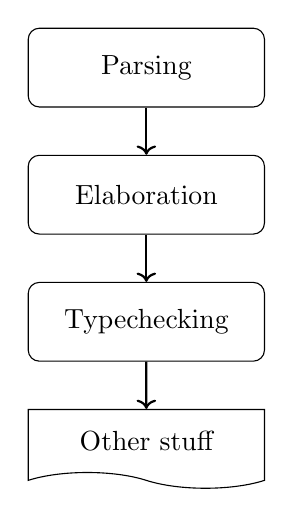
\begin{tikzpicture}[
    start chain=going below,
    every join/.style={arrow},
    node distance=0.6cm
    ]
    \node (s0) [reg,on chain,join] {Parsing};
    \node (s1) [reg, on chain, join] {Elaboration};
    \node (s2) [reg, on chain, join] {Typechecking};
    \node (s3) [end, on chain, join] {Other stuff};
  \end{tikzpicture}
  \begin{tikzpicture}[remember picture, overlay]
    \node [xshift=0.12\paperheight,yshift=0.15\paperheight] at (current page.south west){
      
\includegraphics[width=0.2\paperwidth, keepaspectratio]{mate.png}
    };
  \end{tikzpicture}
  \end{column}
  \begin{column}{0.55\textwidth}
    \begin{itemize}
      \item converts the user code to some very \keyword{faithful internal representation}
      \vspace{0.5em}\item translates to a \keyword{simpler}, potentially more verbose representation
      \vspace{0.2em}\item \keyword{validates} and \keyword{checks} the simpler representation
      \vspace{1em}\item optimisations, environments for code execution, emitting native code, etc.
    \end{itemize}
  \end{column}
  \end{columns}
\end{frame}


\begin{frame}{Parsing Matlab code}
  \begin{columns}
  \begin{column}{0.3\textwidth}
    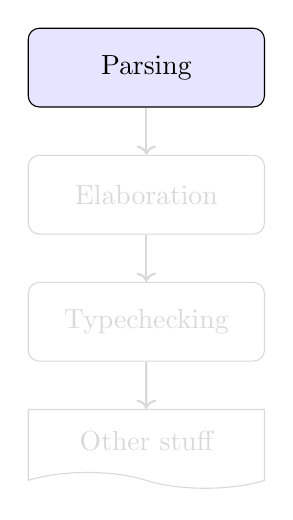
\begin{tikzpicture}[
      start chain=going below,
      every join/.style={fadearrow},
      node distance=0.6cm
    ]
    \node (s0) [highlight, on chain,join] {Parsing};
    \node (s1) [fade, on chain, join] {Elaboration};
    \node (s2) [fade, on chain, join] {Typechecking};
    \node (s3) [fadeend, on chain, join] {Other stuff};
    \end{tikzpicture}
    \begin{tikzpicture}[remember picture, overlay]
      \node [xshift=0.12\paperheight,yshift=0.15\paperheight] at (current page.south west){
        
\includegraphics[width=0.2\paperwidth, keepaspectratio]{mate.png}
      };
    \end{tikzpicture}
  \end{column}
  \begin{column}{0.55\textwidth}
  Parsing actually consists of two phases --- \keyword{lexing} and \keyword{parsing}:
  \begin{itemize}
    \item a \keyword{lexer} converts stream of \keyword{characters} to a stream of \keyword{tokens}, e.g., by grouping digits into numbers, finding comments, etc;
    \item a parser then converts the stream of \keyword{tokens} to an \keyword{abstract syntax tree} - a data structure amenable to further processing
  \end{itemize}
  There is much more to that phase...\\
  Remark: Detecting \lr\ directive happens during lexing, i.e., very early in the pipeline.
  \end{column}
  \end{columns}
\end{frame}

\begin{frame}{Core Type Theory}
  \begin{columns}
  \begin{column}{0.3\textwidth}
    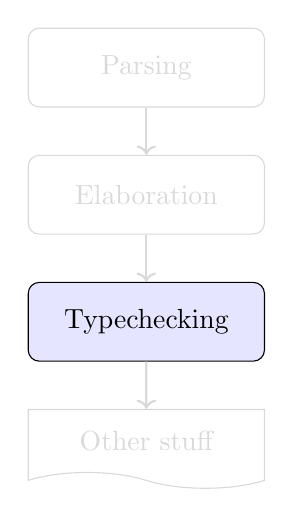
\begin{tikzpicture}[
      start chain=going below,
      every join/.style={fadearrow},
      node distance=0.6cm
      ]
      \node (s0) [fade, on chain,join] {Parsing};
      \node (s1) [fade, on chain, join] {Elaboration};
      \node (s2) [highlight, on chain, join] {Typechecking};
      \node (s3) [fadeend, on chain, join] {Other stuff};
    \end{tikzpicture}
    \begin{tikzpicture}[remember picture, overlay]
      \node [xshift=0.12\paperheight,yshift=0.15\paperheight] at (current page.south west){
        
\includegraphics[width=0.2\paperwidth, keepaspectratio]{mate.png}
      };
    \end{tikzpicture}
  \end{column}
  \begin{column}{0.55\textwidth}
    The algorithmic implementation of the rules of our type system.
    \begin{itemize}
      \item can report any typing errors during compilation
      \item but can also be delayed until program execution, as in \ma
      \begin{itemize}
        \item to the peril of the user
      \end{itemize}
    \end{itemize}
  \end{column}
\end{columns}
\end{frame}

\begin{frame}{A Tour of Types: Unit type}
\end{frame}

\begin{frame}{A Tour of Types: Free Abelian Groups}

\end{frame}


\begin{frame}{A Tour of Types: Matrices}

\end{frame}

\begin{frame}{Elaborating Matlab expressions to CoreTT}

\end{frame}


\begin{frame}[fragile]{Elaborating Assignments}
  \begin{lstlisting}[escapechar=@, language=Matlab, xleftmargin=10em, gobble=4]
    %> n@\tikzmark{ndecl}@ :: int
    n = 5;
    x = n
    %> typeof x
  \end{lstlisting}
  \mycallout<0>{ndecl}{see a variable declaration $n$; invent the type }
\end{frame}

\end{document}
%%% Local Variables:
%%% mode: latex
%%% TeX-master: t
%%% End:
